\documentclass[addpoints]{exam}

\usepackage[table]{xcolor}
\usepackage{amsmath}
\usepackage{amssymb}
\usepackage{hyperref}
\usepackage{pythonhighlight}
\usepackage{titling}
\usepackage{listings}
\usepackage{subfiles}
\usepackage{xcolor}
\usepackage{forest}
\usepackage{tikz} 
\usepackage{tikz-qtree}

\definecolor{codegreen}{rgb}{0,0.6,0}
\definecolor{codegray}{rgb}{0.5,0.5,0.5}
\definecolor{codepurple}{rgb}{0.58,0,0.82}
\definecolor{backcolour}{rgb}{0.95,0.95,0.92}


\lstdefinestyle{mystyle}{
    backgroundcolor=\color{backcolour},   
    commentstyle=\color{orange},
    keywordstyle=\color{red},
    numberstyle=\tiny\color{codegray},
    stringstyle=\color{violet},
    basicstyle=\small\ttfamily,
    breakatwhitespace=false,         
    breaklines=true,                 
    captionpos=b,             
    keepspaces=true,                 
    numbers=left,                    
    numbersep=5pt,                  
    showspaces=false,                
    showstringspaces=false,
    showtabs=false,                  
    tabsize=4
}

\lstset{style=mystyle}


% Header and footer.
\pagestyle{headandfoot}
\runningheadrule
\runningfootrule
\runningheader{CS 412 Algorithms, Spring 2023}{Homework 1}{\theauthor}
\runningfooter{}{Page \thepage\ of \numpages}{}
\firstpageheader{}{}{}

\boxedpoints
\printanswers

\newcommand\cg{\cellcolor{lightgray}}

\title{Homework 1\\ CS 412 Algorithms: Design and Analysis}
\author{q1-team-2}  % replace with your team name without the brackets, e.g. q1-team-420
\date{Habib University | Spring 2023}

\begin{document}
\maketitle

\begin{questions}

	\question
	Horner's method computes a polynomial of degree $n$ as follows.
	\[
		\sum_{i=0}^n a_ix^i = a_0 + x(a_1 + x(a_2 + x(a_3 + \cdots x(a_{n-1}+xa_n)\cdots)) )
	\]
	An algorithm to compute a polynomial using this method is given below.
	\begin{lstlisting}[language=Python]
Horner(A, n, x):
	# A contains the coefficients
	p = 0
	for i = n downto 0:
		p = A[i] + x * p
	return p
	\end{lstlisting}
	\begin{parts}
		\part[5] Is the algorithm correct? Provide a counterexample if it is not, or prove using a loop invariant if it is.
		\part[5] Derive the time complexity of this algorithm?
	\end{parts}

	\begin{solution}
		\begin{parts}
			\part The algorithm is correct. We can prove this using induction and loop invariant. The loop invariant is \(\displaystyle p_k = \sum_{i=0}^{k} a_{n-i}x^{k-i}\), where \(k\) represents the \(k\)th itteration of the loop. For notation we have written \(p\) as \(p_k\) meaning that \(p\) at \(k\)th itteration. Our propositional function would be,
			\[P(k): p_k = \sum_{i=0}^{k} a_{n-i}x^{k-i},\; 0 \leq k \leq n\]
			We would apply induction on \(k\) to show that it is indeed a loop invariant. We can prove that the loop invariant holds at the start of the loop by showing that it holds for \(k=0\). We have,
			\[p_0 = \sum_{i=0}^{0} a_{n-i}x^{0-i} = a_{n-0}x^{0} = a_{n}x^{0} = a_{n}\]
			which is indeed the case. We can also prove that the loop invariant holds at the end of the loop by showing that it holds for \(k+1\), with an assumption that it holds for \(k\) (inductive hyposthesis). We have,
			\begin{align*}
				p_{k+1} & = \sum_{i=0}^{k+1} a_{n-i}x^{k+1-i}                      \\
				        & = a_{n-k-1}x^{k+1-k-1} + \sum_{i=0}^{k} a_{n-i}x^{k+1-i} \\
				        & = a_{n-k-1} + x\sum_{i=0}^{k} a_{n-i}x^{k-i}             \\
				p_{k+1} & = a_{n-k-1} + x \cdot p_k
			\end{align*}
			which is indeed the case.
			\part The time complexity of the algorithm is,
			\[T(n) = \Theta(n)\]
		\end{parts}
	\end{solution}

	\question Derive the closed form solution of each of the following recurrence relations.
	\begin{parts}
		\part[5] $\displaystyle T(m,n) = T\left(\frac{m}{2}, \frac{n}{2}\right) + \Theta(m+n), T(1, n) = T(m, 1) = c$.
		\part[5] $\displaystyle T(m,n) = T\left(m, \frac{n}{2}\right) + \Theta(m), T(1, n) = \Theta(n), T(m, 1) = \Theta(m)$.
	\end{parts}
	\begin{solution}
		We would solve these equations itteratively,
		\begin{parts}
			\part \begin{equation}
				\begin{aligned}
					T(m,n)          & = T\left(\frac{m}{2}, \frac{n}{2}\right) + \Theta\left(m+n\right)                                                                            \\
					\implies T(m,n) & = T\left(\frac{m}{4}, \frac{n}{4}\right) + \Theta\left(\frac{m}{2}+\frac{n}{2}+m+n\right)                                                    \\
					\implies T(m,n) & = T\left(\frac{m}{8}, \frac{n}{8}\right) + \Theta\left(\frac{m}{4}+\frac{n}{4}+\frac{m}{2}+\frac{n}{2}+m+n\right)                            \\
					\vdots                                                                                                                                                         \\
					\implies T(m,n) & = T\left(\frac{m}{2^i}, \frac{n}{2^i}\right) + \Theta\left(\frac{m+n}{2^{i-1}} + \cdots + \frac{m+n}{2}+m+n\right)                           \\
					\implies T(m,n) & = T\left(\frac{m}{2^i}, \frac{n}{2^i}\right) + \Theta\left(\left(m+n\right)\left(\frac{1}{2^{i-1}} + \cdots + \frac{1}{2} + 1 \right)\right) \\
					\implies T(m,n) & = T\left(\frac{m}{2^i}, \frac{n}{2^i}\right) + \Theta\left(2\left(m+n\right)\left(1-\frac{1}{2^{i}} \right)\right)                           \\
				\end{aligned}
			\end{equation}
			From here we can have two cases, \(m \leq n\) or \(m > n\). If \(m \leq n\), then we have \(m\) would become \(1\) in \(i\) itterations, that means \(i=\lg{m}\). If \(m > n\), then we have \(n\) would become \(1\) in \(i\) itterations, that means \(i=\lg{n}\). In case of \(m \leq n\), we have,
			\begin{equation}
				\begin{aligned}
					T(m,n) & = T\left(1, \frac{n}{2^i}\right) + \Theta\left(2\left(m+n\right)\left(1-\frac{1}{m} \right)\right) \\
					       & = \Theta(n) + \Theta\left(2\left(m+n\right)\left(1-\frac{1}{m} \right)\right)                      \\
					       & = \Theta\left(n+2\left(m+n\right)\left(1-\frac{1}{m} \right)\right)                                \\
					       & = \Theta\left(n\right)
				\end{aligned}
			\end{equation}
			In case of \(m > n\), we have,
			\begin{equation}
				\begin{aligned}
					T(m,n) & = T\left(\frac{m}{2^i}, 1\right) + \Theta\left(2\left(m+n\right)\left(1-\frac{1}{n} \right)\right) \\
					       & = \Theta(m) + \Theta\left(2\left(m+n\right)\left(1-\frac{1}{n} \right)\right)                      \\
					       & = \Theta\left(m+2\left(m+n\right)\left(1-\frac{1}{n} \right)\right)                                \\
					       & = \Theta\left(m\right)
				\end{aligned}
			\end{equation}

			We can write both cases in one notation as,
			\begin{equation}
				\begin{aligned}
					T(m,n) & = \Theta\left(m+n\right)
				\end{aligned}
			\end{equation}

			\newpage

			\part \begin{equation}
				\begin{aligned}
					T(m,n)          & = T\left(m, \frac{n}{2}\right) + \Theta(m)    \\
					\implies T(m,n) & = T\left(m, \frac{n}{4}\right) + \Theta(2m)   \\
					\implies T(m,n) & = T\left(m, \frac{n}{8}\right) + \Theta(3m)   \\
					\vdots                                                          \\
					\implies T(m,n) & = T\left(m, \frac{n}{2^i}\right) + \Theta(im)
				\end{aligned}
			\end{equation}
			Let \(n=2^i\iff i=\lg{n}\), that means,
			\begin{equation}
				\begin{aligned}
					T(m,n) & = T\left(m, 1\right) + \Theta(m\lg{n}) \\
					T(m,n) & = \Theta(m) + \Theta(m\lg{n})          \\
					T(m,n) & = \Theta(m\lg{n})
				\end{aligned}
			\end{equation}
		\end{parts}
	\end{solution}

	\question[5] What is the set, $O(f(n)) \cap \Omega(f(n))$? Justify your answer.

	\begin{solution}
		We know that,
		\begin{equation*}
			\begin{aligned}
				O(f(n))      & := \left\{g(n) \mid \exists c\in\mathbb{R} \ni g(n) \leq cf(n) \right\} \\
				\Omega(f(n)) & := \left\{g(n) \mid \exists c\in\mathbb{R} \ni g(n) \geq cf(n) \right\}
			\end{aligned}
		\end{equation*}
		Therefore,
		\begin{equation*}
			\begin{aligned}
				O(f(n)) \cap \Omega(f(n)) & = \bigg\{g(n) \bigg| \bigg(\exists c_0\in\mathbb{R} \ni g(n) \leq c_0f(n)\bigg) \land \bigg(\exists c_1\in\mathbb{R} \ni g(n) \geq c_1f(n) \bigg) \bigg\} \\
				                          & = \bigg\{g(n) \bigg| \exists c_0,c_1\in\mathbb{R} \ni c_1f(n) \leq g(n) \leq c_0f(n) \bigg\}                                                              \\
				                          & = \Theta(f(n))                                                                                                                                            \\
			\end{aligned}
		\end{equation*}
		\hfill \(\square\)
	\end{solution}

	\question[5] We are given the series, $f(n) = \sum_{i=0}^nar^i$, where $|r|>0$. Show that
	\[
		f(n) =
		\begin{cases}
			\Theta(r^n) & r > 1 \\
			\Theta(n)   & r = 1 \\
			\Theta(1)   & r < 1 \\
		\end{cases}
	\]

	\begin{solution}
		We would devide our proof into two cases,
		\subsection*{Case I: \(r=1\)}
		It is trivial to show,
		\begin{equation}
			\begin{aligned}
				\left(f(n) = \sum_{i=0}^n ar^i\right) \land \left(r=1\right) & \implies f(n) = \sum_{i=0}^n a = an \\
				                                                             & \implies f(n)=\Theta(n)
			\end{aligned}
		\end{equation}

		\subsection*{Case II: \(r > 1\)}
		We know that,
		\[\forall i < j, r^{i} < r^{j}\]
		This implies that,
		\begin{equation}
			\begin{aligned}
				a                                            & < ar^{n+1}                        \\
				ar                                           & < ar^{n+1}                        \\
				ar^2                                         & < ar^{n+1}                        \\
				\vdots                                                                           \\
				ar^n                                         & < ar^{n+1}                        \\
				\hline
				\therefore a+ar+ar^2+\cdots+ar^n             & < a(n+1)r^{n+1}                   \\
				f(n)                                         & < a(n+1)r^{n+1}                   \\
				\implies \underbrace{a}_{c_0}r^{n} \leq f(n) & < \underbrace{a(n+1)r}_{c_1}r^{n} \\
				\implies f(n)                                & = \Theta(r^n)
			\end{aligned}
		\end{equation}

		\newpage

		\subsection*{Case III: \(r < 1\)}
		We know that,
		\[\forall i < j, 0 < r^j < r^i < 1\]
		This implies that,
		\begin{equation}
			\begin{aligned}
				a                                                   & \leq a                         \\
				ar                                                  & < a                            \\
				ar^2                                                & < a                            \\
				\vdots                                                                               \\
				ar^n                                                & < a                            \\
				\hline
				\therefore a+ar+ar^2+\cdots+ar^n                    & < a(n+1)                       \\
				f(n)                                                & < a(n+1)                       \\
				\implies \underbrace{\frac{1}{1-r}}_{c_0}(1) < f(n) & < \underbrace{a(n+1)}_{c_1}(1) \\
				\implies f(n)                                       & = \Theta(1)
			\end{aligned}
		\end{equation}
		\hfill\(\square\)
	\end{solution}

	\question[5] To highlight the CS strength at Habib University, NSOs are planning a particular formation on the stairs from the library to the music room. One new student stands on the top stair and places their hands on the shoulders of up to two new students on the next stair. Each of them, in turn, places their hands on the shoulders of up to two students on the next stair, and so on, all the way to the last stair. There is at least one person on every stair.

	Numbering the top stair as $0$ and the bottom one as $n$, express the total number of new students standing on all the stairs using recurrence relations. Solve the recurrences, and state what they mean for the number of students.

	\begin{solution}
		The students will be in a formation like this
		\begin{center}
			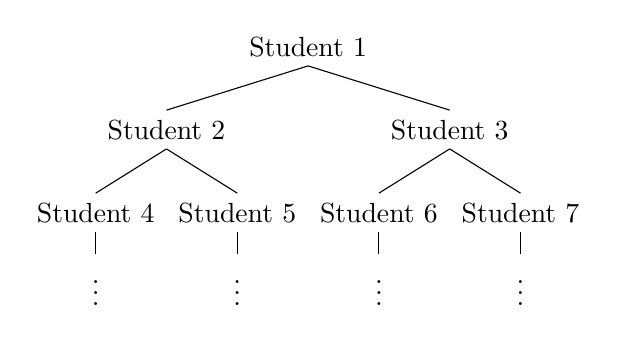
\begin{tikzpicture}
				\Tree [.\node{Student 1};
				[.\node{Student 2};
				[.\node{Student 4};[.\node{\vdots};]]
				[.\node{Student 5};[.\node{\vdots};]]]
				[.\node{Student 3};
				[.\node{Student 6};[.\node{\vdots};]]
				[.\node{Student 7};[.\node{\vdots};]]]
				]
			\end{tikzpicture}
		\end{center}

		So we have a binary tree like formation. We look at the first few terms to see a pattern
		\begin{align*}
			T(0) & = 1                            \\
			T(1) & = 1 + 2         & = T(0) + 2^1 \\
			T(2) & = 1 + 2 + 4     & = T(1) + 2^2 \\
			T(3) & = 1 + 2 + 4 + 8 & = T(2) + 2^3 \\
			\vdots                                \\
			T(n) & = T(n-1) + 2^n
		\end{align*}

		So we have our recurrence relation as:
		\[T(n) = T(n-1) + 2^n\]
		We see a telescoping series here. We would rewrite the equation and add it for different values of \(n\).
		\begin{equation*}
			\begin{aligned}
				T(n) - T(n-1)   & = 2^n                          \\
				T(n-1) - T(n-2) & = 2^{n-1}                      \\
				\vdots                                           \\
				T(1) - T(0)     & = 2^1                          \\\\\hline\\
				T(n) - T(0)     & = 2^n + 2^{n-1} + \cdots + 2^1 \\
				T(n) - 1        & = \sum_{i=1}^{n} 2^i           \\
				T(n)            & = 1 + \sum_{i=1}^{n} 2^i       \\
				T(n)            & = \sum_{i=0}^{n} 2^i
			\end{aligned}
		\end{equation*}

		\textbf{Claim:} \[\forall n \in \mathbb{N}, \;\;\sum_{i=0}^n 2^i = 2^{n+1} - 1\]
		\\\\\textbf{Proof 1:} We show this by basic algebraic manipulation,
		\begin{equation*}
			\begin{aligned}
				S_n            & = \sum_{i=0}^n 2^i                           \\
				\implies 2S_n  & = 2^1 + 2^2 + \cdots + 2^n + 2^{n+1}         \\
				\implies - S_n & = 2^0 \pm 2^1 \pm \cdots \pm 2^{n-1} \pm 2^n \\\\\hline\\
				2S_n - S_n     & = 2^{n+1} - 1                                \\
				\implies S_n   & = 2^{n+1} - 1
			\end{aligned}
		\end{equation*}
		\\\\\textbf{Proof 2:} We show this by mathematical induction
		\\\textbf{Base case:} Let $n = 0$
		$$\sum_{i=0}^0 2^i = 2^0 = 2^{0+1} - 1 = 1$$
		\textbf{Induction hypothesis:}
		\\Let $n = k$
		\\Assume that the following relation holds for $n = k$
		$$\sum_{i=0}^k 2^i = 2^{k+1} - 1$$
		\textbf{induction Step:}
		\\Let $n = k+1$
		\\So we have that
		$$\sum_{i=0}^{k+1} 2^i = 2^{k+1} + \sum_{i=0}^{k} 2^i $$
		From our induction hypothesis we have that $\sum_{i=0}^k 2^i = 2^{k+1} - 1$
		\\So we have that
		$$\sum_{i=0}^{k+1} 2^i = 2^{k+1} + 2^{k+1} - 1 = 2\times 2^{k+1} - 1 = 2^{k+2} - 1$$
		So we have that $\sum_{i=0}^{k+1} 2^i = 2^{k+2} - 1$ which is what we wanted.
		\\So we have that $\sum_{i=0}^n 2^i = 2^{n+1} - 1$ for all $n \in \mathbb{N}$
		\\So now from above expression for $T(n)$ we have
		$$T(n) = T(n-1) + 2^n = \sum_{i=0}^n 2^i = 2^{n+1} - 1$$
		\\So now from above expression for $T(n)$ we have
		$$T(n) = T(n-1) + 2^n = \sum_{i=0}^n 2^i = 2^{n+1} - 1$$
		Now we have a closed form solution for $T(n)$:
		$$T(n) = 2^{n+1} - 1$$
		For $n$ stairs the number of students will be $2^{n+1} - 1$
	\end{solution}

	\newpage

	\question Given a list of $n$ student IDs representing all the check-ins in a day at all the card machines at Habib, we want to extract the unique IDs. in each of the following situations.
	\begin{parts}
		\part[5] Provide a divide-and-conquer algorithm for the purpose that does not use sorting and has a time complexity of $O(n^3)$.
		\part[5] Provide a divide-and-conquer algorithm for the purpose that may use sorting and has a time complexity of $O(n\lg n)$.
	\end{parts}
	For each algorithm, justify its running time and argue that it is correct.

	\begin{solution}
		\begin{parts}
			\part

			\lstinputlisting[language=Python]{q6a.py}

			The recurrence relation describing the time complexity of this algorithm will be
			$$T(n) = 3T\left(\frac{n}{3}\right) + \Theta(n)$$
			Using Master Theorem we have that $T(n) = \Theta(nlg n)$. So the time complexity of the algorithm is in $O(n\log{n})$ and $O(n\log{n}) \subset O(n^3)$ so algorithm is in $O(n^3)$.
			\\\\The algorithm is correct as we recursively divide the array into 3 parts, then we compute the unique ids in each part then for combining the our solution of the subproblems,
			we maintain a list a list of unique elements, let $U$ be the list of unique ids, $A$ be the list of unique ids in the first part of the array, $B$ be the list of unique ids in the second part of the array,
			$C$ be the list of unique ids in the third part of the array, for each id in $A$ if that id is not in $U$ we add it in $U$, for each id in $B$ if that id is not in $U$ we add it in $U$, for each id in $C$ if that id is not in $U$ we add it in $U$.
			This way $U$ hold the unique ids of all 3 parts, therefore the unique ids of the entire array.
			\part

			\lstinputlisting[language=Python]{q6b.py}

			The recurrence relation describing the time complexity of this algorithm will be
			$$T(n) = 2T\left(\frac{n}{2}\right) + \Theta(n)$$
			Using Master Theorem we have that $T(n) = \Theta(n\lg{n})$. So the time complexity of the algorithm is in $O(n\log{n})$.
			\\\\The algorithm is correct as we recursively divide the array into 2 parts, then we compute the unique ids in each part then for combining the our solution of the subproblems,
			we maintain a list a list of unique elements, let $U$ be the list of unique ids, $A$ be the list of unique ids in the first part of the array, $B$ be the list of unique ids in the second part of the array,
			for each id in $A$ if that id is not in $U$ we add it in $U$, for each id in $B$ if that id is not in $U$ we add it in $U$.
			This way $U$ hold the unique ids of both parts, therefore the unique ids of the entire array.
		\end{parts}
	\end{solution}

	\newpage

	\question[5] The \textit{Towers of Habib} game is played on $n$ pegs with an abundant supply of disks. Players take turns placing disks on the pegs. Any number of disks may be placed on any peg provided that the resulting number of disks on the peg is more than the number of disks on the left peg, if any, and less than those on the right peg, if any. Once all the pegs are occupied, the \textit{Aadaab} state occurs if peg number $i$ has $i$ disks on it. At this point, everyone says, ``Aadaab'', to each other.

	Provide an $O(\lg n)$ divide-and-conquer algorithm to detect if the game is currently in the \textit{Aadaab} state. Argue that it is correct and has the required time complexity.

	\begin{solution}
		\\\textbf{Lemma 1:} Given a state of Tower of Habib game such that all pegs are occupied, the game is in \textit{Aadaab} state if and only if the first peg has 1 disk on it.
		\\\textbf{Proof of lemma 1:}
		\\Let $S$ be a ordered list that represents the state of the game, where $i^{\text{th}}$ element of $S$ represents how many disk are on $i^{\text{th}}$ peg.  We denote the number of elements of $S$ as $|S|$ and $i^{\text{th}}$ element of $S$ as $S[i]$.
		\\First we prove that if the game is in Aadaab state then the first peg has 1 disk on it.
		Suppose the game is in \textit{Aadaab} state, then we know there exists some $i$, where $1\leq i\leq |S|$, such that $S[i] = i$.
		\\As all pegs are occupied we know that no element of $S$ is equal to $0$, we also know that \\$\forall i \in \{2,..., |S|\}, \;S[i-1] < S[i] < S[i+1]$.
			So if $S[i] = i$ then for the elements from 1 to $S[i-1]$ we only have numbers from 1 to $i-1$ that they can have, as if we have a number greater than that then some peg will have more disks then the peg on its right.
			\\So the only satifying placement of disks on pegs 1 to $i-1$ under these conditions is that $\forall j \in \{1,..., i-1\}, S[j] = j$, so peg 1 will have 1 disk on it.
			\\Now for the converse if we have that all pegs are occupied and the first peg as 1 disk on it so we have found our $i$ such that $S[i] = i$, as $S[1] = 1$, so the game is in \textit{Aadaab} state.
			\\\\Now we argue that given a state of the game we cannot find if all the pegs are occupied in $O(\log n)$ time. Let $S$ be a list representing the state of the game, if some peg is empty, then there is some $i$, $1 \leq i \leq |S|$, such that $S[i] = 0$.
			\\so then then the sorted condition $\forall i \in \{2,..., |S|\}, \;S[i-1] < S[i] < S[i+1]$ is not satified that is to say $\exists i \in \{2,..., |S|\}, S[i-1] > S[i]$. So the problem now becomes given a list $S$ which is not sorted does is 0 an element of $S$.
			As under this condition $S$ is not sorted anymore, then to search 0 in $S$ we need to check each element of $S$ and compare it with $0$, if it is equal to $0$ then we have found out $0$, if not we keep searching until all elements are checked if all elements are checked and 0 isnt found then we know that 0 doesn't exist in $S$.
			We cannot do this in less than $O(n)$, suppose that there exists some algorithm that searches 0 in $S$ in less time than $O(n)$ then as the algorithm takes less than $O(n)$ steps we know that it skips some element of $S$ and doesnt check if that element is $0$, but what if that element is indeed 0? In an unsorted list we have no garantee that the skipped element isn't 0, so this algorithm will not be correct.
			\\\\So we we cannot see if all the pegs are occupied, to satisfy this questions prompt we will assume that all the pegs are occupied and our algorithm will just see if given that all pegs are occupied is that game in \textit{Aadaab} state?
			\\The following divide and conquer algorithm determines if the game is in \textit{Aadaab} state given that all pegs are occupied:

			\newpage
			\lstinputlisting[language=Python]{toh.py}
			The algorithm runs in $O(\log n)$, as the recurrence relation for the time complexity of the algorithm will be $T(n) = T(n/2) + \theta(1)$,
			using Master Theorem we have that $\log_2 (1) = 0 = d$, so $T(n) = \Theta(n^0 \log n) \subset O(\log n)$.
		\\As for the correctness of the given algorithm, the algorithm recursively, halfs the input list representing the game state, and calls its self on the first half of the list, it keeps recusively calling until there only the first element of the list remains.
		\\From lemma 1 we know that the game is in \textit{Aadaab} state if anf only if the first element is equal to 1, so our algorithm just check if the first element is equal to 1 if it is equal to 1 it outputs true, else it outputs false.

	\end{solution}

	\question[5] In the run-up to \href{https://en.dailypakistan.com.pk/13-Jan-2019/this-pakistani-varsity-will-celebrate-feb-14-as-sister-s-day}{Sisters Day}, CSOs are analyzing the daily number of PDA cases on campus since the start of classes at Habib University in August 2014. Given the data of $n$ days, a \textit{successful} day is one in which the number is not greater than the day just prior, if it exists, or the day just after, if it exists.

	For example, the successful days are highlighted in each of the 3 sample data sets below.

	\begin{tabular}{*{3}{c}}
		\begin{tabular}{*{7}{|c}|}
			\hline
			\cg 3 & 5 & 7 & \cg 2 & 9 & \cg 0 & 1 \\
			\hline
		\end{tabular}
		 &
		\begin{tabular}{*{9}{|c}|}
			\hline
			\cg 8 & 9 & 10 & 11 & 12 & 7 & 6 & 5 & \cg4 \\
			\hline
		\end{tabular}
		 &
		\begin{tabular}{*{6}{|c}|}
			\hline
			10 & 9 & 8 & \cg 7 & \cg 7 & \cg 7 \\
			\hline
		\end{tabular}
	\end{tabular}

	Provide an $O(\lg n)$ divide-and-conquer algorithm to identify a successful day. Argue that it is correct and has the required time complexity.

	\begin{solution}
		The algorithm is as if we are searching for a local minimum in the data. We can use binary search to find the local minimum in $O(\lg n)$ time. The algorithm is as follows:
		\begin{enumerate}
			\item Find the middle element of the data set.
			\item If the middle element is the first or last element, then it is a local minimum.
			\item If the middle element is greater than the element to its left, then the local minimum is in the left half of the data set.
			\item If the middle element is greater than the element to its right, then the local minimum is in the right half of the data set.
			\item If the middle element is less than both its left and right elements, then it is a local minimum.
		\end{enumerate}

		\newpage

		\lstinputlisting[language=C++]{q8.cpp}

		We are doing constant work at each step and each time reducing the size of the problem by half. So the recurrence relation is,
		\[T(n) = T\left(\frac{n}{2}\right) + \Theta(1)\]
		Using the Master Theorem, we have that $a = 1$, $b = 2$, and $f(n) = \Theta(1)$. So, $T(n) = O(\lg n)$.


	\end{solution}

	\question Below, list any and all sources, \href{https://hulms.instructure.com/courses/2616/discussion_topics/29240}{including AI tools}, that you have consulted for any of the problems above. We are interested in learning about unsuccessful attempts just as much as successful ones.

	\begin{solution}

	\end{solution}

\end{questions}

\end{document}
